
\section{The Large Hadron Collider}

The process the Large Hadron Collider (LHC) uses sounds simple when put into common terms. It accelerated protons to speeds very close to the speed of light and collides them in the center of a detector to see what comes out of these collisions. However actually doing this is not simple at all. The theory of special relativity says that a particle can only approach the speed of light. As the protons in the LHC are traveling close to the speed of light it is more useful to use their energy rather than their speed. In addition, mass is often put into units of energy of the speed of light squared making the mass to energy conversion simple. To start this entire process electrons are stripped off of hydrogen gas supplying the protons for the LHC. After this the protons are put into a series of different accelerator each designed to accelerator to protons to higher and higher energies. The first accelerator is the Linac2 linear accelerator, which gets the protons up to 50 MeV. Then they are sent to the Proton Synchrotron Booster which can push them to 1.4 GeV, after which the Proton Synchrotron ring accelerates the protons to 25 GeV. At this point the protons are sorted to control the frequency at which the collisions will occur. The protons are sorted into bunches such that given a fixed point on the LHC a proton bunch passes by every 25ns. Each bunch has about 100 billion protons in it. After sorted into these bunches the protons are sent to the Super Proton Synchrotron where they achieve an energy of 450 GeV. Finally, the protons are fed into the LHC where they will be accelerated to their highest energy.

% Some figure showing the CERN accelerator complex?
\begin{figure}
\centering
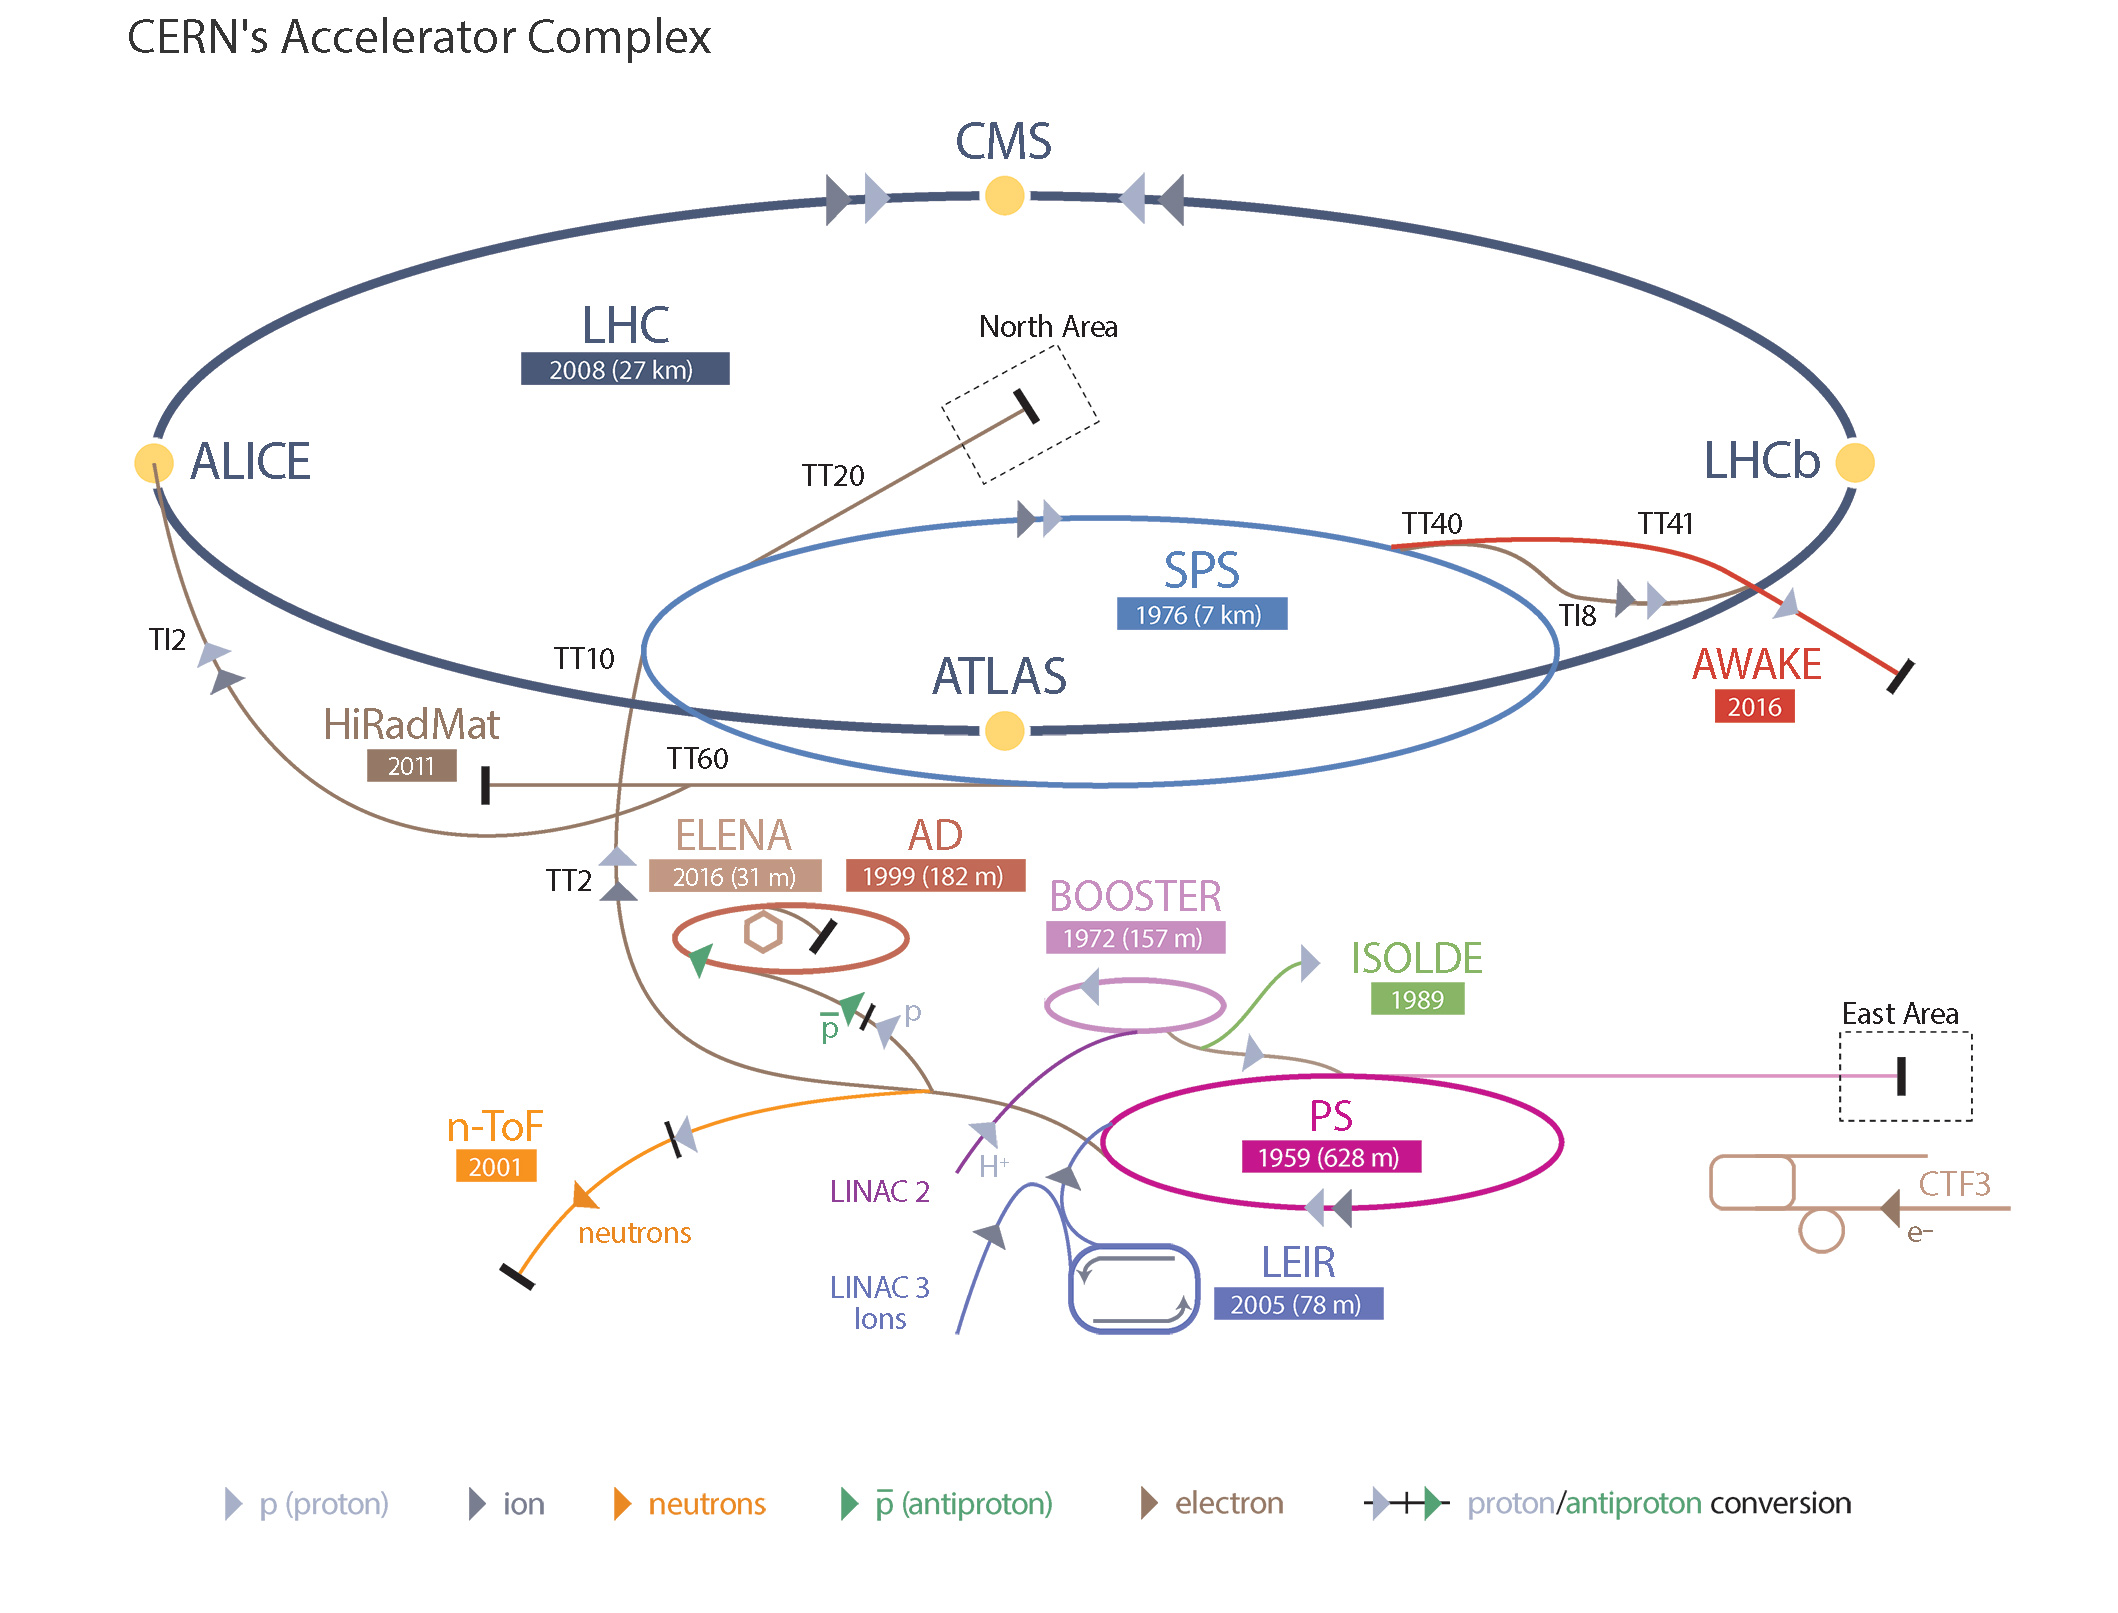
\includegraphics[width=0.8\linewidth]{Figures/acceleratorcomplex.jpg}
\caption{Chain of accelerators feeding into the LHC}
\label{fig:acceleratorcomplex}
\end{figure}

When the LHC has accelerated its particles to its peak energy it collides the particles in the middle of four different detectors. LHCb, ALICE, ATLAS, and CMS are the names of the four detectors that were built to study collisions supplied by the LHC. The CMS detector is the one I worked on during my undergraduate career, and is discussed in detail below.

\section{The CMS Detector}
The CMS detector is designed to detector particles coming out of the proton-proton collisions supplied by the LHC. As many different types of particles come out of these collisions the CMS detector is split up into several different sub-detectors. Going from the closest to the collision point outward, first is the silicon tracker. This is responsible for measuring the total energy of the particles in the detector which is important for reconstructing the events using conservation of energy. Next is the Electromagnetic Calorimeter which is responsible for detecting a myriad of charged particles such as photon, and electrons. Then there is the Hadron Calorimeter which is responsible for detector hadrons, which are particles made up of quarks, such as protons neutrons and pions. These calorimeters work by covering the possible directions out of the collision with scintillator tiles. When the particles hit these tiles they lose some of their energy depositing light proportional to the energy of the particle. The particle will eventually stop having lost all of its energy giving us a reading on its total energy. Finally, are the muon chambers. Muons are interesting particles because while they are heavy particles that will decay they have long enough lifetimes to make it through the detector. In addition, they tend to not be stopped by the detector like the two prior calorimeters almost always stop the particles they detect. Since there is a magnetic field encompassing the detector and the muons have a charge they will curve as they pass through the muon chambers. While not completely stopping the muons will give a reading in the chambers showing its path of travel. By measuring the curve of this path of travel we can measure the momentum. By combining the the data from all the different sub detectors we can get a picture of almost all of the particles that came out of the collision. There are exceptions such as neutrinos which tend to pass through anything leaving no trace. Nevertheless we are able to use this to recreate what exactly came out of the collision, which allows us to find evidence of particles like the top quark which decays so quickly it does not even make it to the detector.

% change to different picture
\begin{figure}
\centering
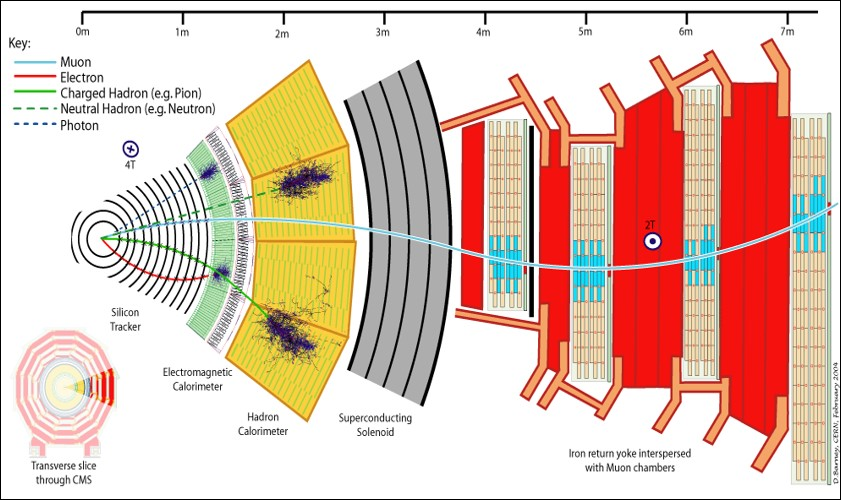
\includegraphics[width=\linewidth]{Figures/CMSlayout.jpg}
\caption{A slice of the CMS detector highlighting the different sub-detectors and showing different particles and where they are stopped}
\label{fig:CMSlayout}
\end{figure}

\subsection{Hadron Calorimeter}
One of the main jobs of the calorimeter is to measure the energy of the of the incident particle. When the particle hits the scintillator tile and loses energy it emits photons into the tile proportional to the amount of energy it lost. To measure the energy of the particle we just have to count up the photons it deposited. To do this we put a fiber around the edges of the tile so that any photons deposited will run into this fiber. The fiber is designed so that once it enters the fiber it will have total internal reflection on the edges meaning it will stay inside the fiber. The fiber then runs to a silicon photomultiplier (SiPM). The SiPM is designed to take light signals and covert them to charge signals. The light from the scintillator tiles is shined on what is called the pixel face of the SiPM. This is just a circular array of really small pixels. There are about 33000 pixels on a 3.3 mm diameter pixels face. When an individual photon hits one of the pixels on the pixel face it causes a capacitor to fire off a particular amount of charge. The total output charge of the SiPM is the sum of all of the pixels output charge. Theoretically one just needs to sum up the total amount of output charge of the SiPM and one can count the number of incident photons since each pixel will fire off a set amount of charge. The counting of the number of incident photons will give a measurement of the incident particles energy. There are some things that make the SiPMs reading not so simple. SiPMs are non-linear devices meaning the total output charge of the SiPM does not necessarily increase linearly with the number of incident photons. In fact, experiments have shown that graphing the number of incident photons vs the SiPM output charge it looks more like a square root function rather than a straight line. At low incident photon count on the order of 1000 photons the SiPM is very close to a linear device but as the incident number of photons increases the output charge does not increase at the same rate.

\begin{figure}
\centering
\includegraphics[width=0.6\linewidth]{Figures/Tile.png}
\caption{A picture of a scintillator tile with the optical fiber around the edges.}
\label{fig:Tile}
\end{figure}

There are three main section to the HCAL. There is the Hadron Barrel (HB), which surrounds the beam-line like the edge of a cylinder, the Hadron End-cap (HE), which caps off the cylinder made by HB. These two parts make a cylinder which has the beam-line going through the center and the collision point in the center. Lastly there is the Hadron Front-cap (HF) which is shaped like HE but is located much further away from the collision point closer to the Muon chamber distance. To describe the geometry of the detector we use a coordinate system related to spherical coordinates with the origin being the collision point and polar angle of 0 being along the beam-line. Phi is the azimuthal angle and Eta is related to the polar angle by $\eta = -\ln(\tan(\theta/2))$ which gives a value of 0 perpendicular to the beam-line and $\pm\infty$ along the beam-line. Usually these coordinates are arranged into discrete integers values denoted iphi and ieta, which are arranged such that a scintialltor tile covers one ieta and one iphi as shown in figure~\ref{fig:Depth} but there are exception to this. For the distance from the beam-line depth is used which is also a discrete value but there are often more than one scintillator tiles in a single depth. 

% HCAL layouts
\begin{figure}
\centering
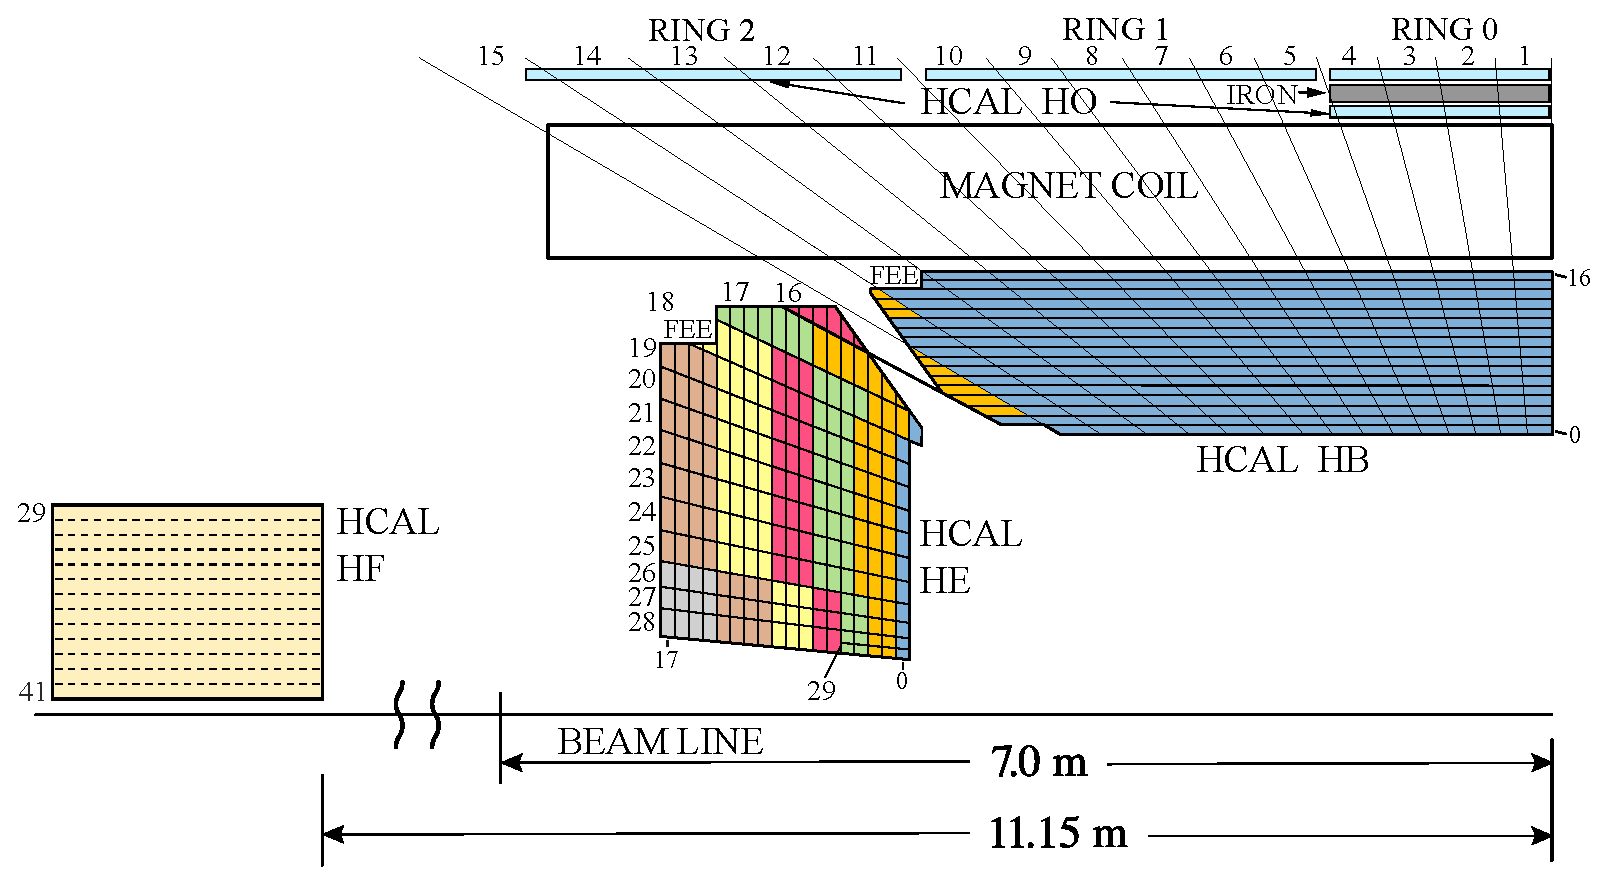
\includegraphics[width=\linewidth]{Figures/Depthsegmentation.pdf}
\caption{Layout of the HCAL showing a single iphi slice of HE HB and HF. Each box represents a scintillator tile}
\label{fig:Depth}
\end{figure}

\subsection{Silicon Photomultipliers}
There are several factors that contribute to SiPM non-linearity but the two main ones are cross talk and saturation. Cross talk is when a pixel is activated by a photon there is a chance that this activated pixel could activate some of its neighboring pixels artificially increase the output charge of the SiPM. When the photon hits a pixel it excites an electron causing an electron cascade and charge to flow. This excited electron has a chance to emit an IR photon which could go in any direction. If it hits one of the neighboring pixels it could activate it just like an incident photon. Saturation is when a pixel is hit in rapid succession by multiple photons. When a pixel is hit by a photon it discharges its capacitor which is the source of its output charge. After it fires it needs some time on the order of 10 nanoseconds to recharge its capacitor. If the pixel is hit it simply fires off whatever charge it has in its capacitor at the time which could be reduced from its normal charge. Given that the SiPM has about 33000 pixels on its pixel face when the number of incident is on the order of 1000 this effect is insignificant but particles can produce much more photons where this effect can be much more significant. The non-linear properties of the SiPM makes it a bit harder to get accurate measurements, but there are ways to study them which will allow us to compensate for these affects.

\begin{figure}
\centering
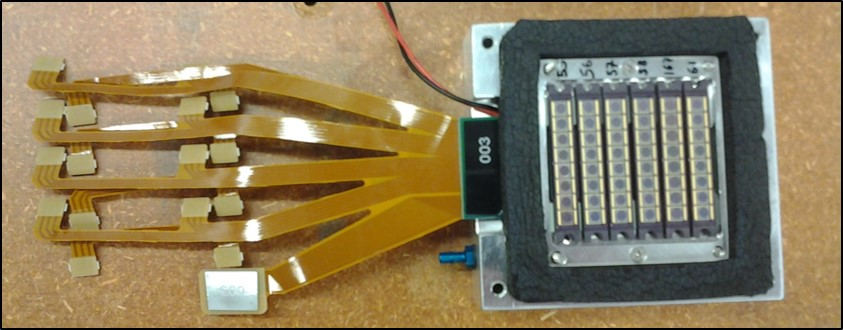
\includegraphics[width=\linewidth]{Figures/SiPM.jpg}
\caption{A picture of a Silicon Photomultiplier}
\label{fig:SiPM}
\end{figure}

\section{Test Beam}
SiPMs are one of the main features of new electronics that are being installed in the CMS detector. These new readout modules main function is to take the signals from the detector, the light signals from incident particles and convert them to digitized charge signals which can be later stored and analyzed. There are several new features with these new readout modules such as new charge integrator and encoder (QIE) chips, but the main subject of my work was the SiPMs. The main way the SiPM non-linearity and other things about the new readout modules are being study is with a test beam. The test beam is a linear particle beam that comes from the SPS accelerator when it does not feed into the LHC. The particles from this beam are not at the energies of the protons in the LHC but they are much easier to make and control. There are several different experiments that use this beam but the HCAL has a mock test stand that can be moved into the path of the beam when experiments need to be run. The CMS detector is 100 meters underground and is in a cavern that due to radiation and tight enclosures makes the detector difficult to access. Though modifications and maintenance can be during shutdowns this is not the ideal way to run tests on new electronics. The test stand at the test beam location called H2 can be easily accessed observed and is on ground level. In addition the energy and particle type of the beam can be easily controlled. The test stand is designed to be similar to a portion of the HCAL on CMS. As such when we shoot particles from the test beam at the test stand with the new electronics on it we can measure its response to experiment like conditions. Using this test beam we can shoot particles like pions at the test stand which has the new readout module installed and look at the response. We can vary the energy of the pions which should increase the number of incident photons on the SiPMs in the readout modules and measure their response to this. In this way we can find the non-linearity of the SiPMs and create a correction curve based on this.

Because we are looking for statistical in the data we need to take a lot of data. This means we take runs with several thousand events or particle hitting the test stand and take several of these runs to ensure high statistics. On the other hand this means we want o minimize the amount of information stores per event so we can store a lot of them. One of the key systems that helps this is the trigger system. In the path of the beam before the test stand we put scintillator tiles not designed to stop the particle entire but rather to send a generic signal to the control room. A total of four tiles were placed in the path of the beam. When we saw signals from these tiles we know that a particle is coming from the beam. This serves as our trigger signal. The trigger signal then goes to the back-end electronics that stores the data from the detector. In this way we only store data coming during the short amount of time on the order of 25 nanoseconds when we know their is relevant information coming. There is also a ready signal that goes from the back-end electronics to the trigger. Since a particle may come before the back-end electronics are finished storing the relevant data a trigger signal that comes without the ready signal will simply be ignored.

Although built to be similar to the HCAL on the CMS detector the test stand is smaller and has some differences. When looking at the data from the teat beam it is important to be sure that the e-map, which traces the channels that receive the data to the actual scintillator tiles on the detector, is correct. To account for the difference between the test stand and the HCAL a new e-map needed to be created. With an accurate e-map we can create an accurate picture of the incident particles hitting the test stand. The test beam allows us to control the energy and type of particles incident on the test stand. This allows us to study things like SiPM non-linearity as we can look at the output of the SiPMs under something like $50 \GeV$ pions then increase to energy to something like $150 \GeV$ and compare the different responses. However the particle does not deposit its energy in a single scintillator tile. For something like a pion it will lose a part of its energy with each scintillator tile it hits and eventually be stopped by the detector but its total energy will be spread throughout the detector. Since each particle in the beam has roughly the same energy and we can isolate the event of a single particle hitting the detector we are to find energy lost in each scintillator tile but looking at the complete picture of the detector. 

SiPM non-linearity is not the only thing that is being researched using the test beam. In the CMS detector particles come so fast that the signals of individual particles blend together. In the test beam the particles are more spread out so it is easier to isolate the signal of individual particles. This makes it easier to extract the pulse shape of the readout modules which is the shape of the output charge vs time. It is also important to see if the pulse shape changes significantly under different circumstances such as higher or lower energies. Using the pulse shape of the readout modules we can then extract the individual signals in the CMS detector.

\section{SiPM simulation}
In addition to studying the new electronics with the test beam, we also did a SiPM simulation which could use theoretical signal from the detector and give the SiPMs response to them. When the light from the detector goes to the SiPM a Y11 light mixer is used so that the light is spread across the pixel face. The light mixer has a unique shape in which is shines the light onto the pixel face. Using a mathematical representation of this pulse shape we can simulate how light is shined on the pixel face. We can then create a virtual pixel face that has accurate geometric representation of the pixel face. Each of these virtual pixels could be activated by the incoming Y11 light pulse and would respond by firing off a set amount of charge just like an actual SiPM would. When these pixels are activated they also have a certain probability to activate a neighboring pixel which will simulate the cross talk of the SiPM. Each pixel also has a recharge rate so if it is hit in rapid succession it will fire with a reduced amount of charge emulating the saturation effect. Using this simulation we easily adjust the number of input photons and get very good details of the SiPM response. We can also easily turn different things off to see how significant individual effects are. This simulation is capable of producing more fine tuned data and in greater quantities than test beam data. In addition, it is able to simulate situations that are not possible in the test beam. On the other hand the accuracy of this simulation is heavily dependent on the data we input into it.

Since the program can simulate the non-linearity effects of the SiPM, we can use theoretical inputs to the SiPM to study its effects. The light a particle deposits in a scintillator tile can vary in time the Y11 light mixer ensures that the input light pulse shape remains constant. This means to change energy of the incident particle we just have to increase the number of photons in the input pulse while keeping the same shape. The output of the virtual SiPM is normalized so if the simulation was a completely linear device its output "charge" should exactly equal the number of input photons. 

\begin{figure}
\centering
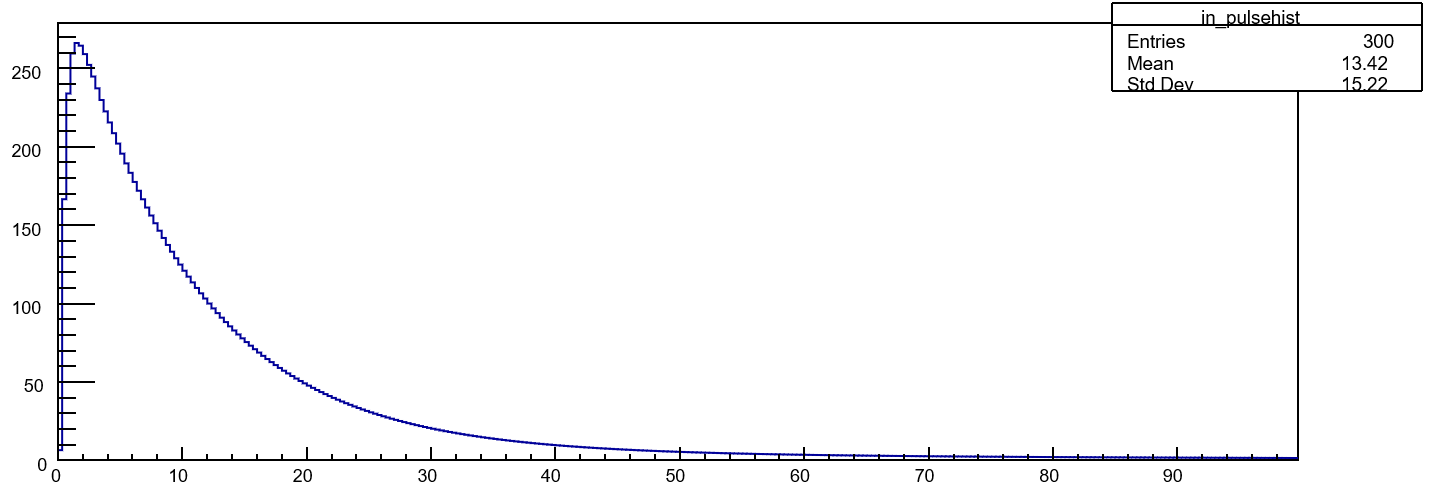
\includegraphics[width=\linewidth]{Figures/Y11.png}
\caption{A graph of the Y11 pulse shape with nanoseconds on the x axis and number of incident photons on the y axis}
\label{fig:Y11}
\end{figure}

